\chapter{Transfer Function Optimization Using Visibility-Weighted Saliency}

\section{Introduction}
Volume visualization is an effective means of discovering meaningful features in volume data sets.
Both the exterior and interior of structures can be revealed simultaneously in a semi-transparent manner by specifying opacity values for the features in transfer functions.
Features can be intensity intervals in 1D transfer functions, rectangular or other shapes in 2D or higher-dimensional transfer functions.

In the specification of transfer functions for volume visualization, users often have a rough idea of how clear and opaque each feature should be and then adjust the opacity value of the features accordingly.
However, the relationship between the opacity of features and the saliency of the features in the final image is not linear.
The saliency of a feature in the final image depends on the opacity value assigned to the feature as well as the neighborhood of the feature and view-dependent occlusion of the feature.

Therefore, it is desirable to have an automated method to assist the user in the design of transfer functions. In this chapter, we propose an optimization approach to automatically refine a user-defined transfer function towards target saliency levels specified by the user.

\section{Related Work}
% line search \cite{armijo_minimization_1966}
% conjugate gradient descent \cite{shewchuk_introduction_1994}

%-------------------------------------------------------------------------
\section{Method}
In Chapter~\ref{visibility-weighted_saliency}, visibility-weighted saliency was proposed as a measure of visual saliency of features in volume rendered images, in order to assist users in choosing suitable viewpoints and designing effective transfer functions to visualize the features of interest. In this chapter, we describe a transfer function optimization approach based on the visibility-weighted saliency metric, which indicates the perceptual importance of voxels and the visibility of features in volume rendered images.

The approach described in Chapter~\ref{transfer_function_refinement} is an automated method of optimizing transfer functions, based on the intensity distribution of voxels in the volume data set. However, this approach does not take into account the spatial distribution of voxels and the viewpoint of the visualization. Visibility-weighted saliency, on the other hand, takes into account both of these two aspects. The visibility-weighted saliency consists of two component fields, i.e. saliency field and visiblity fields. Saliency fields are essentially difference of Gaussians, which include the information of local neighborhoods of voxels, and visibility fields are computed from opacity contribution of voxels to volume rendered images, which indicate viewpoint dependent occlusions of the voxels.

Constraints are introduced in the search of the parameter space. Only the opacity of features would be changed in the transfer function domain. The definition of features (e.g. the data intervals) and the colors of features remain the same.
These constraints are based on the assumption that the user has explored the volume data and set up the transfer function according to his/her needs. Our algorithm aims to help the user reduce occlusion while preserving the user's knowledge or judgments of the data set.

\subsection{Objective Function}
Users define target importance values for each feature defined in the transfer function domain.
Our transfer function optimizer adjusts the transfer function to match the visibility-weighted saliency with the user-defined target saliency values.
Multiple saliency fields computed from different appearance attributes can be combined together in order to represent different aspects of the visual saliency of voxels.
In our implementation, brightness and saturation are used respectively to compute visibility-weighted saliency fields and define the weighted sum of the two sets of feature saliency as visibility-weighted feature saliency.
The objective function $ f $ is defined as the root mean square of the differences of the visibility-weighted saliency and target importance of each feature.
\[ f=\sqrt{ \frac{\sum_{i=1}^{n} (W_{i}-t_{i})^{2}}{n} } 
\addtag \]
where $ W_{F}=u_{1}W_{F}(O_{b},i,\sigma)+u_{2}W_{F}(O_{s},i,\sigma) $ is the visibility-weighted saliency of feature $ i $, and $ t_{i} $ is the user-defined importance of feature $ i $. These user-defined saliency values are normalized and they add up to 1, in other words, $ t_{i} \in [0.1] $ and $ \sum_{i=1}^{n} t_{i} = 1 $.

As previously described in Section~\ref{weighted_feature_saliency}, multiple saliency fields computed from different appearance attributes can be combined together in order to represent different aspects of the visual saliency of voxels.
In our implementation, $ W_{F}=u_{1}W_{F}(O_{b},i,\sigma)+u_{2}W_{F}(O_{s},i,\sigma) $ is a weighted sum of visibility-weighted saliency values computed using brightness and saturation of voxels respectively, and $ u_{1} $ and $ u_{2} $ are weights of the two appearance attributes.

However, the visibility-weighted saliency $ W_{i} $ is not a variable that can be directly modified. Instead, $ W_{i} $ is a complicated function of the color and opacity of voxels in feature $ i $ and is also influenced by the viewpoint of rendering. A visibility-weighted saliency field is a combination of a visibility field and a saliency field. The saliency field is a view-independent field based on the color of every voxels in the volume data set, while the visibility field is a view-dependent field computed from the opacity contribution of every voxels to the final image when rendered from a certain viewpoint.

The computation of visibility fields is non-trivial. In order to compute a visibility field, a slice-based rendering is performed on a series of quads which are parallel to the viewing plane, one for each slice.
Subsequently, the visibility values are computed by subtracting the accumulated opacity of the previous slice from that of the current slice. After collecting the visibility values of all voxels, the visibility field can be constructed. The details of visibility fields were previously described in Section~\ref{visibility_fields}.

The evaluation of the objective function is computational expensive. However, in an iterative optimization, the visibility field and visibility-weighted saliency have to be recompute at each step after the feature opacity value are updated.

\subsection{Parameter Space}
We use a nucleon data set to demonstrate how the visibility-weighted saliency of features change when the feature opacity values change. As displayed in Figure~\ref{fig:nucleon_naive}, three features are defined in the transfer function for the nucleon data set.

The dimension of the parameter space is the same as the number of features defined by the user. In this case, three features are defined for the nucleon data set. The opacity of each feature is mapped to an axis in the parameter space. Therefore, the opacity values of the 3 features are mapped to $ x, y, z $ axes of a 3D scalar field. Figure~\ref{fig:nucleon_densityplot} displays three 3D scalar fields, one for each feature, to provide an intuitive overview of the relationship between the feature opacity values and the visibility-weighted saliency values.

Feature 1 (the purple structure in Figure~\ref{fig:nucleon_naive}) is the exterior of the nucleon data set, the visibility-weighted saliency of this feature is shown in the 3D scalar fields in the same color at the left in Figure~\ref{fig:nucleon_densityplot}.
The visibility-weighted saliency of feature 1 increases as its opacity increases, as shown in the 3D scalar fields that the brightness and opacity increase along $ x $ axis. Similar patterns also appear in the other 2 scalar fields, the visibility-weighted saliency of feature 2 (the red structure in Figure~\ref{fig:nucleon_naive}) and feature 3 (the green structure in Figure~\ref{fig:nucleon_naive}) also increase as their opacity increase.
%Thus it is reasonable to assume that the visibility-weighted saliency of a feature is a monotonic function of its opacity.

Moreover, feature 1 is the exterior of the nucleon, its visibility-weighted saliency is almost not influenced by the opacity of other features. On the other hand, the visibility-weighted saliency of feature 2 is influenced by both the opacity of feature 1 and feature 2. In addition, the visibility-weighted saliency of feature 3 is drastically influenced by the opacity of feature 1, feature 2 and feature 3, as feature 3 is an interior structure and can be easily occluded by the other 2 features.

In order to demonstrate the distribution of the objective function in the parameter space $ x \in [0,1] $, $ y \in [0,1] $ and $ z \in [0,1] $, we sample the parameter space with sampling interval $ 0.1 $, from 0 to 1 along each axis. There are 11 sampling points along each axis, which results in 1331 sampling points in the parameter space. In Figure~\ref{fig:nucleon_parameterspace}, the parameter space is rendered as a density plot with a temperate color map which gradually changes from orange to blue.

\begin{figure}
\centering
	\begin{minipage}{.35\textwidth}
	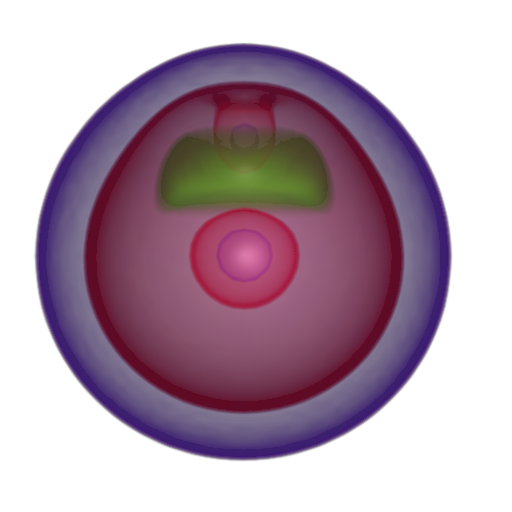
\includegraphics[width=1\linewidth]{images/nucleon_naive}
	\end{minipage}~
	\begin{minipage}{.2\textwidth}
	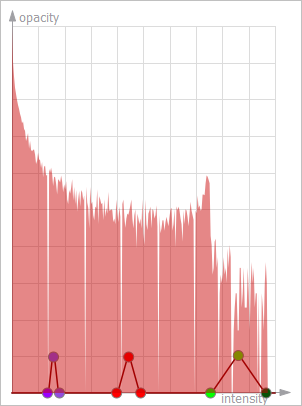
\includegraphics[width=1\linewidth]{images/tf_nucleon_naive}
	\end{minipage}
	\caption{A nucleon data set \cite{website:Voreen_datasets_2013} (left) with a transfer function of equal opacity values to the 3 features (right)}
	\label{fig:nucleon_naive}
\end{figure}

\begin{figure}
	\centering
	\begin{minipage}{.3\textwidth}
		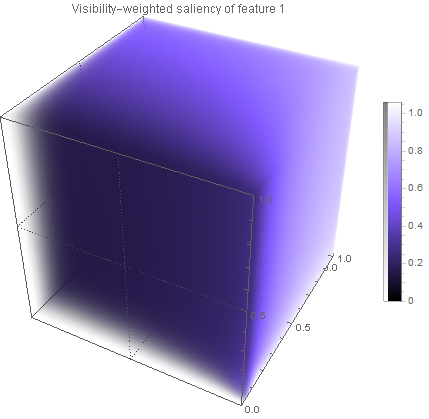
\includegraphics[width=1\linewidth]{images/nucleon_strong_red_densityplot1}	
	\end{minipage}~
	\begin{minipage}{.3\textwidth}
		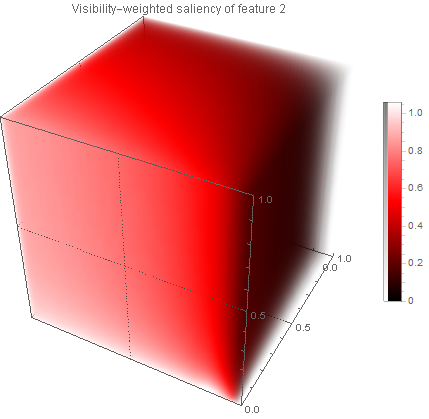
\includegraphics[width=1\linewidth]{images/nucleon_strong_red_densityplot2}	
	\end{minipage}
	\begin{minipage}{.3\textwidth}
		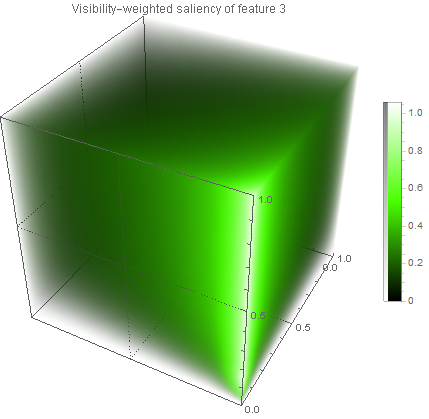
\includegraphics[width=1\linewidth]{images/nucleon_strong_red_densityplot3}	
	\end{minipage}
	\caption{Visibility-weighted saliency of the 3 features are mapped to brightness and opacity of the 3D fields at the left, middle and right respectively. The visibility-weighted saliency of feature 2 (red) is affected by both the opacity of feature 1 (purple) and feature 2. The visibility-weighted saliency of feature 3 (green) is affected by the opacity of feature 1, feature 2 and feature 3.}
	\label{fig:nucleon_densityplot}
\end{figure}

\begin{figure}
	\centering
	\begin{minipage}{.6\textwidth}
		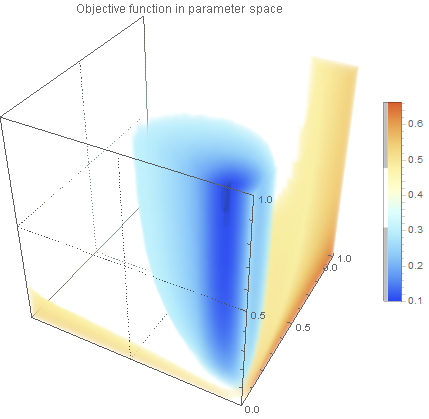
\includegraphics[width=1\linewidth]{images/nucleon_strong_red_parameterspace}
	\end{minipage}
	\caption{Each position (x, y, z) in the parameter space represents 3 features with opacity values (x, y, z). The value of the objective function $ f $ (with \{0.1, 0.3, 0.6\} as target) is mapped to the color in the parameter space (with sampling interval $ 0.1 $). Only the high and low values are visible and the data range in the middle is set to transparent.}
	\label{fig:nucleon_parameterspace}
\end{figure}

\subsection{Optimization Algorithm}
The gradient descent algorithm is employed in our transfer function optimizer.
Gradient descent is a first-order optimization algorithm. It is based on the observation that if a function $ f(x) $ is defined and differentiable in a neighborhood of a point $ x_{1} $, then $ f(x) $ decreases fastest in the direction of the negative gradient of the function \cite{chong_introduction_2013}.

Given a continuously differentiable function $ f(x) $ with $ x \in \mathbb{R}^{n} $, let $ x_{k} $ be the current iteration point and $ g_{k}=g(x_{k})= \nabla f(x_{k}) $ be the gradient of $ f(x) $ at $ x_{k} $. The gradient descent method defines the next iteration point by
\[ x_{k+1}=x_{k}- \alpha_{k} g_{k} , k \geq 0 \]
for $ \alpha_{k} $ small enough, then $ f(x_{k+1}) \leq f(x_{k}) $. The gradient varies as the iteration proceeds, tending to zero as it approaches a local minimum. When the gradient decreases, the iteration step sizes also decrease. So hopefully the sequence $ {x_{k}} $ converges to the desired local minimum after performing the iteration.

In gradient descent methods, we can either take very small step sizes and reevaluate the gradient at every steps, or take large steps each time. If the step size is too small, it may end up in a laborious situation that the objective function converges very slowly. If the step size is too large, it results in a more zigzag path and may have the risk of missing the local minimum and thus cannot converge.

\subsection{Estimating Search Directions}
In each step of the optimization, the search direction $ g_{k} $ has to be updated. 
As previously discussed, the visibility-weighted saliency of a feature increases as its feature opacity increases. 
%The visibility-weighted saliency of a feature is a monotonic function of the opacity of the feature. 
However, the relationship between the visibility-weighted saliency and the opacity of a feature also depends the viewpoint of rendering and the spatial distribution of voxels of every features in the volume data set. An exact derivative of the visibility-weighted saliency with respect to the opacity of the feature cannot be determined in advance.

In the following subsections, three different methods for estimating gradients or search directions are described.

\subsubsection{Backward Difference}
The first method is to estimate the gradient with a backward difference divided by a small step.
\[ \frac{\nabla_{d}[f](x)}{d}=\frac{f(x)-f(x-d)}{d} \]
where $ d $ is nonzero number.
When $ d $ is small, the backward difference divided by $ d $ approximates the derivative. Assuming that $ f $ is differentiable, the error in this approximation can be derived from Taylor's theorem.
\[ \frac{\nabla_{d}[f](x)}{d}-f'(x)=\mathcal{O}(d) \to 0 , \; as \; d \to 0 \]
The evaluation of the objective function $ f $ is very computational expensive. In our implementation, a small step size $ d $ is adopted, therefore the backward difference can calculated from values of the objective function, visibility-weighted saliency and step positions of the last iteration. In this case, no extra evaluation of the visibility-weighted saliency and the objective function is required.

\subsubsection{Derivatives with Backward Difference}
The partial derivative of the objective function $ f $ with respect to $ x_{i} $ is
\[ \frac{\partial f}{\partial x_{i}} = \frac{\partial f}{\partial W_{i}} \frac{\partial W_{i}}{\partial x_{i}} \]
where $ x_{i} $ is the opacity and $ W_{i} $ is the visibility-weighted saliency of feature $ i $.

The partial derivative $ \frac{\partial f}{\partial W_{i}} $ can be solved from the objective function $ f $. However, $ \frac{\partial W_{i}}{\partial x_{i}} $ cannot be determined without knowledge the actual volume data set. The backward difference is used here to approximate $ \frac{\partial W_{i}}{\partial x_{i}} $, hence we have
\[ \frac{\partial W_{i}}{\partial x_{i}} \approx \frac{\nabla_{d}[W_{i}](x_{i})}{d} \]
Similarly, the backward difference can calculated from previous values of the visibility-weighted saliency and step positions.

Furthermore, if the function $ W_{i} $ of $ x_{i} $ is approximately a linear function, the partial derivative $ \frac{\partial W_{i}}{\partial x_{i}} $ becomes constant and could be replaced by an empirical constant $ b_{i} $. In this case, the gradient of the objective function with respect to the visibility saliency is used instead, which should be more computationally efficient.
\[ \frac{\partial f}{\partial x_{i}} \approx \frac{\partial f}{\partial W_{i}} b_{i} \]
In our implementation, $ b_{i}=1 $ is used and this yields desirable results.

\subsubsection{Newton's Method Using Backward Difference}
Newton's method, which is an iterative method for finding the roots of a differentiable function, can be used to find a minimum or maximum of a function. Because the derivative is zero at a minimum or maximum, minima and maxima can be found by applying Newton's method to the derivative. Hence we have
\[ x_{k+1}=x_{k}- \frac{f'(x_{k})}{f''(x_{k})} \]
This iteration equation gives a similar form of gradient descent, thus we can use $ \frac{f'}{f''} $ in our optimization algorithm as the search direction.

The first-order derivative can be estimated by backward difference of the objective function $ f $, and the second-order derivative $ f'' $ can be estimated by backward difference of the first-order derivative $ f' $.
\[ \frac{f'}{f''} 
\approx \dfrac{ \frac{\nabla_{d}[f](x_{i})}{d} }{ \frac{\nabla_{d}[f'](x_{i})}{d} }
= \frac{ \nabla_{d}[f](x_{i}) }{ \nabla_{d}[f'](x_{i}) } \]

\subsubsection{Results of the Estimation Methods}
We have tested the gradient estimation methods discussed above with several volume data sets with various step sizes.
In the preliminary results, we found these methods work with small step sizes. As the step size increase, using $ \frac{\nabla_{d}[f](x)}{d} $ and $ \frac{\partial f}{\partial W_{i}} \frac{\nabla_{d}[W_{i}](x_{i})}{d} $ as search directions would be unstable. While using $ \frac{\partial f}{\partial W_{i}} b_{i} $ and $ \frac{ \nabla_{d}[f](x_{i}) }{ \nabla_{d}[f'](x_{i}) } $ as search directions would be still stable even when the step sizes are large. In addition, with the same step size, using $ \frac{\partial f}{\partial W_{i}} b_{i} $ as the search direction would converge fastest among these methods.

\subsection{Adaptive Step Size with Line Search}
Performing gradient descent with a small step size may result in converging too slowly and require a lot of evaluations of the objective function, which is rather expensive to compute in our situation. Various approaches have been proposed regarding the choices of step sizes, which lead to various gradient algorithms \cite{yuan_step-sizes_2008}.

The line search strategy is an iterative approach that adapts the step size in gradient descent in order to achieve a reduction in the objective function while still making sufficiently fast progress.
\[ h( \gamma)=f(x_{k}+\gamma g_{k}) \]
where $ g_{k} $ is the descent direction and $ x_{k} $ is the current point at the $ k$-$th $ iteration.

There are two type of approaches of line search, exact line search and inexact line search \cite{vrahatis_class_2000}.
Exact line search chooses the next iteration point by achieving the least objective function value. However, despite the optimal properties, exact line search often behave poorly and tend to zigzag in two orthogonal directions, which usually implies deteriorations in converge \cite{zhou_gradient_2006}.
On the contrary, inexact line search only loosely find a sufficient decrease of the objective function along the descent direction.

The inexact line search we used in our implementation is as follows.

\begin{enumerate}
	\item Set initial iteration count $ i=0 $ and set $ n $ to the maximum iteration count.
	\item Check whether $ f(x_{k}+\gamma_{i+1} g_{k}) < f(x_{k}+\gamma_{i} g_{k}) $ where $ \gamma_{i}=2^{i} $
	\item If so and $ i<n-1 $, $ i=i+1 $ and repeat Line 2, otherwise terminate the line search.
\end{enumerate}

The step size $ \gamma_{n} $ is chosen after the above line search procedure.
This strategy does not find the exact minimum along the line direction, instead it yields reasonable results and descents much faster than using fixed step sizes.

\subsection{Parallel Line Search}
The classical gradient descent is a sequential algorithm. In its iterative procedure, the next iteration takes the result from the previous iteration as input.
However, the line search at each iteration can be computed parallel to accelerate the optimization. This idea is particularly useful in our transfer function optimization, because the most expensive computation in our transfer function optimization is the evaluation of visibility-weighted saliency, which is required in the evaluation of the objective function at each iteration.

In this section, we propose a parallel line search strategy, which evaluates the objective function at different candidate points in parallel along the line search direction. With this parallel approach, the computing power of modern multi-core processors can be better exploited to accelerate the transfer function optimization. Specifically, parallel line search launches multiple threads to perform the line search. Each thread computes the visibility-weighted saliency and the objective function at a candidate point. Subsequently, the results at all the candidate points are aggregated and the candidate point with the minimum objective function value is chosen as the next step.

The parallel line search is shown as follows.

\begin{enumerate}
	\item Generate a list of step sizes $ S= \{ \gamma_{0},\gamma_{1},...,\gamma_{n-1} \} $ where $ \gamma_{i}=2^{i} $
	\item Evaluate $ f(x_{k}+\gamma_{i} g_{k}) $ in parallel for each $ \gamma_{i} $ in $ S $
	\item Find the index $ i $ of the minimum $ f(x_{k}+\gamma_{i} g_{k}) $, then $ \gamma_{i} $ is the chosen step size.
\end{enumerate}

The mechanism of the parallel line search is sightly different from the sequential line search. In the sequential line search, if the current candidate point does not meat the condition, the line search is terminated and the next candidate point would not be evaluated. By contrast, the parallel line search would always evaluate all the candidate points and pick the one with least value of the objective function. However, these two methods would have the same behavior if the objective function is a convex function.

The parallel line search strategy would introduce extra overhead of starting and terminating threads. Moreover, the number of threads should not exceed the number of cores of the processor, otherwise multiple threads have to share the same core and this would cause performance impact. The parallel line search is beneficial only when the evaluation of the objective function is more expensive than the parallel overhead.
In our case, the evaluation of the objective function is very computational expensive. It requires to compute the visibility fields, which in turn requires to perform a pass of slice-based volume rendering.

%-------------------------------------------------------------------------
\section{Results and Discussions}

*** work in progress ***

Search paths in parameter space
Figure~\ref{fig:nucleon_parameterspace_path}

Objective function
Figure~\ref{fig:nucleon_strong_red_rms}

Visibility-weighted saliency of each feature
Figure~\ref{fig:nucleon_strong_red_saliency}

Opacity of each feature
Figure~\ref{fig:nucleon_strong_red_opacity}

Before optimization
Figure~\ref{fig:nucleon_strong_red}

After optimization
Figure~\ref{fig:nucleon_strong_red_optimized_fixed}

\begin{figure}
	\centering
	\begin{minipage}{.35\textwidth}
		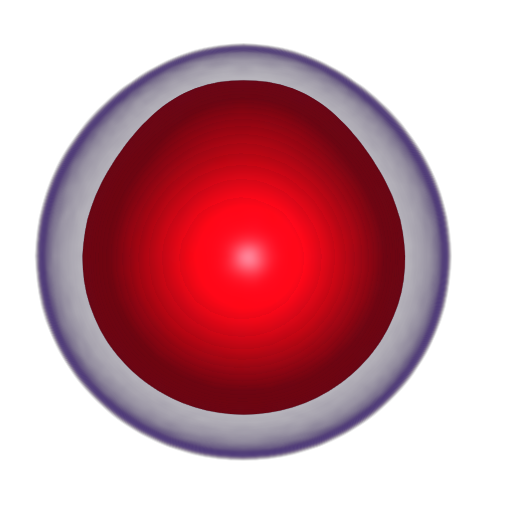
\includegraphics[width=1\linewidth]{images/nucleon_strong_red}
	\end{minipage}~
	\begin{minipage}{.2\textwidth}
		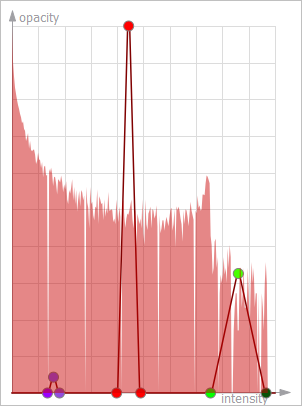
\includegraphics[width=1\linewidth]{images/tf_nucleon_strong_red}	
	\end{minipage}~
	\begin{minipage}{.4\textwidth}
		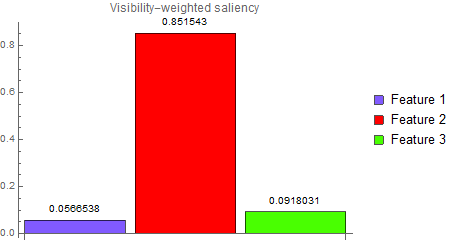
\includegraphics[width=1\linewidth]{images/nucleon_strong_red_visibility_saliency_weighted_chart}
	\end{minipage}
	\caption{Before optimization, the transfer function strongly emphasizes the red feature, which occludes the green feature inside. (Left: the volume rendered image of the nucleon data set; Middle: the transfer function; Right: the visibility-weighted saliency histogram)}
	\label{fig:nucleon_strong_red}
\end{figure}

\begin{figure}
	\centering
	\begin{minipage}{.35\textwidth}
		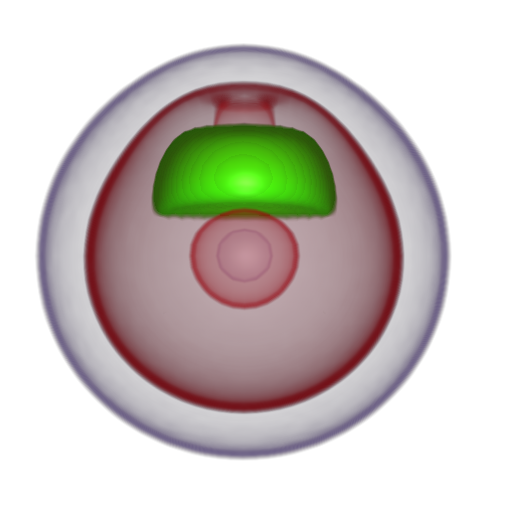
\includegraphics[width=1\linewidth]{images/nucleon_strong_red_optimized_fixed}
	\end{minipage}~
	\begin{minipage}{.2\textwidth}
		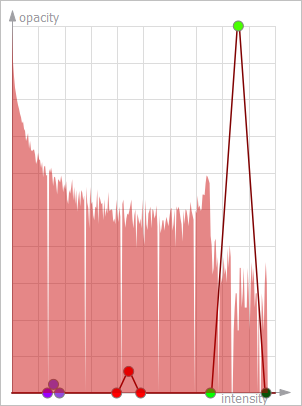
\includegraphics[width=1\linewidth]{images/tf_nucleon_strong_red_optimized_fixed}
	\end{minipage}~
	\begin{minipage}{.4\textwidth}
		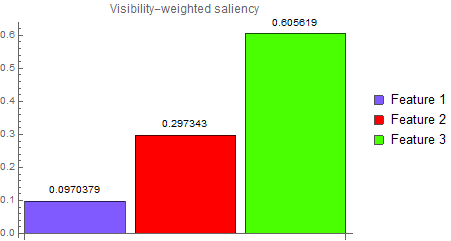
\includegraphics[width=1\linewidth]{images/nucleon_strong_red_optimized_fixed_visibility_saliency_weighted_chart}
	\end{minipage}
	\caption{After optimization to target \{0.1, 0.3, 0.6\}, all the 3 features are visible and the green feature inside is particularly emphasized. (Left: the volume rendered image of the nucleon data set; Middle: the transfer function; Right: the visibility-weighted saliency histogram)}
	\label{fig:nucleon_strong_red_optimized_fixed}
\end{figure}

\begin{table}[h]
\begin{tabular}{ l | l c r }
	& Fixed step size & Line search & Parallel line search \\
	\hline
	Time (seconds) & 1.91 & 0.83 & 0.55 \\
	Iterations to converge (at 0.01) & 37 & 4 & 4 \\
\end{tabular}
\caption[Table caption text]{Performance of the 3 optimization approaches on the nulceon data set ($ 41 \times 41 \times 41 $)}
\label{table:nucleon_table}
\end{table}

\begin{table}[h]
	\begin{tabular}{ l | l c r }
		& Fixed step size & Line search & Parallel line search \\
		\hline
		Time (seconds) & 18.05 & 6.59 & 3.31 \\
		Iterations to converge (at 0.01) & 47 & 4 & 4 \\
	\end{tabular}
	\caption[Table caption text]{Performance of the 3 optimization approaches on the tooth data set ($ 140 \times 120 \times 161 $)}
	\label{table:tooth_table}
\end{table}

\begin{table}[h]
	\begin{tabular}{ l | l c r }
		& Fixed step size & Line search & Parallel line search \\
		\hline
		Time (seconds) & 120.38 & 59.01 & 33.41 \\
		Iterations to converge (at 0.01) & 47 & 6 & 6 \\
	\end{tabular}
	\caption[Table caption text]{Performance of the 3 optimization approaches on the CT-Knee data set ($ 379 \times 229 \times 305 $)}
	\label{table:CT-Knee_table}
\end{table}

\begin{figure}
	\centering
	\begin{minipage}{.9\textwidth}
		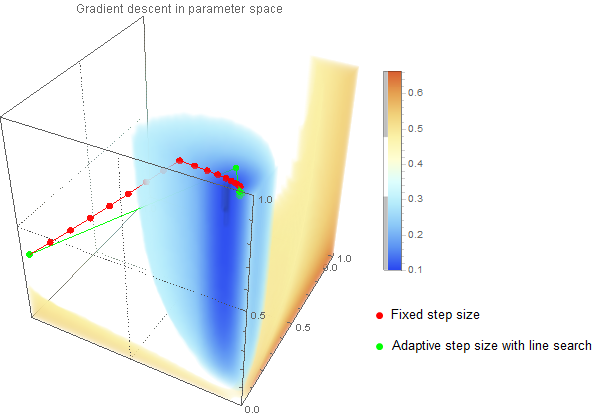
\includegraphics[width=1\linewidth]{images/nucleon_strong_red_parameterspace_path}
	\end{minipage}
	\caption{The steps of gradient descent methods with fixed step size and adaptive step size are shown in the parameter space in Figure~\ref{fig:nucleon_parameterspace} (the step size is 0.1)}
	\label{fig:nucleon_parameterspace_path}
\end{figure}

\begin{figure}
	\centering
	\begin{minipage}{.33\textwidth}
		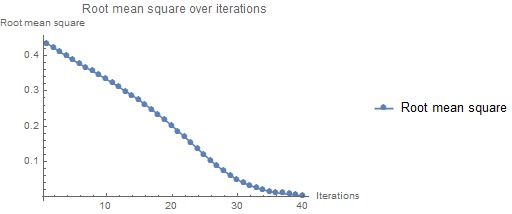
\includegraphics[width=1\linewidth]{images/nucleon_strong_red_rms_fixed}
	\end{minipage}~
	\begin{minipage}{.33\textwidth}
		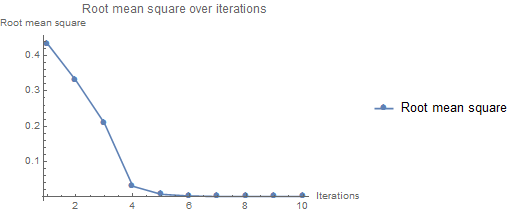
\includegraphics[width=1\linewidth]{images/nucleon_strong_red_rms_linesearch}
	\end{minipage}~
	\begin{minipage}{.33\textwidth}
		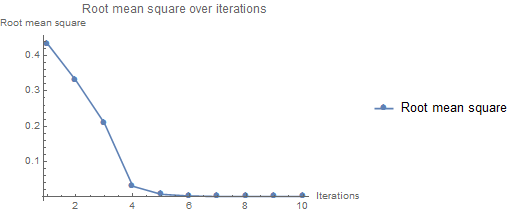
\includegraphics[width=1\linewidth]{images/nucleon_strong_red_rms_parallelsearch}
	\end{minipage}
	\caption{How the objective function change over iterations respectively in the 3 optimization approaches. (Left: fixed step size; middle: line search; right: parallel line search)}
	\label{fig:nucleon_strong_red_rms}
\end{figure}

\begin{figure}
	\centering
	\begin{minipage}{.33\textwidth}
		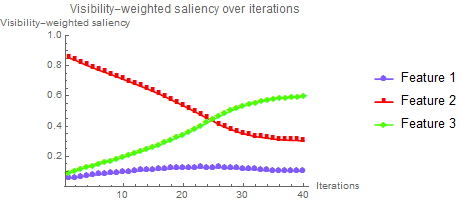
\includegraphics[width=1\linewidth]{images/nucleon_strong_red_saliency_fixed}
	\end{minipage}~
	\begin{minipage}{.33\textwidth}
		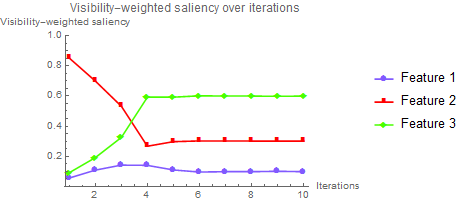
\includegraphics[width=1\linewidth]{images/nucleon_strong_red_saliency_linesearch}
	\end{minipage}~
	\begin{minipage}{.33\textwidth}
		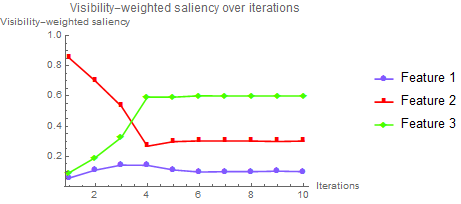
\includegraphics[width=1\linewidth]{images/nucleon_strong_red_saliency_parallelsearch}
	\end{minipage}
	\caption{How the visibility-weighted saliency of each feature change over iterations respectively in the 3 optimization approaches. (Left: fixed step size; middle: line search; right: parallel line search)}
	\label{fig:nucleon_strong_red_saliency}
\end{figure}

\begin{figure}
	\centering
	\begin{minipage}{.33\textwidth}
		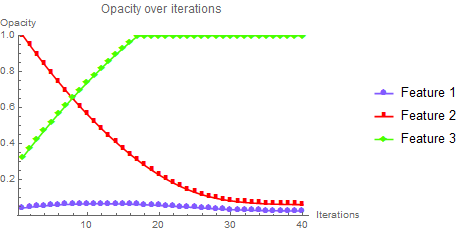
\includegraphics[width=1\linewidth]{images/nucleon_strong_red_opacity_fixed}
	\end{minipage}~
	\begin{minipage}{.33\textwidth}
		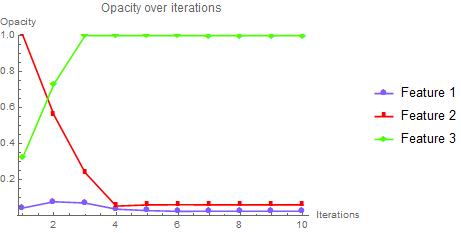
\includegraphics[width=1\linewidth]{images/nucleon_strong_red_opacity_linesearch}
	\end{minipage}~
	\begin{minipage}{.33\textwidth}
		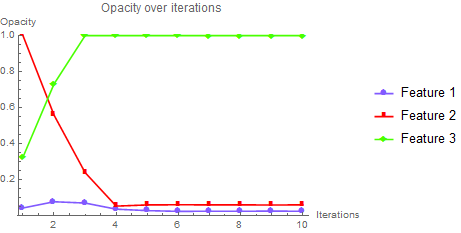
\includegraphics[width=1\linewidth]{images/nucleon_strong_red_opacity_parallelsearch}
	\end{minipage}
	\caption{How the opacity of each feature change over iterations respectively in the 3 optimization approaches. (Left: fixed step size; middle: line search; right: parallel line search)}
	\label{fig:nucleon_strong_red_opacity}
\end{figure}

%-------------------------------------------------------------------------
\section{Conclusions}
This chapter proposes a novel transfer function optimization approach using the visibility-weighted saliency metric.
With this approach, the design of transfer functions becomes more intuitive. This approach allows the user to directly set target visibility-weighted saliency for features of interest and then the transfer function is automatically refine to match the visibility-weighted saliency of the features with the user-defined targets.
This approach has proven to be effective over several volume data sets.
